\documentclass[12pt]{beamer}
\usetheme{Madrid}
\usecolortheme{default}

\usepackage{amsmath}
\usepackage{siunitx}
\usepackage{graphicx}
\usepackage{booktabs}
\usepackage{tikz}
\usetikzlibrary{arrows.meta, positioning, decorations.pathmorphing}

\sisetup{per-mode=symbol, separate-uncertainty=true}

\title[Speed of Sound Dependence]{DIY Lab: Speed of Sound Dependence on\\Temperature and Pressure}
\author[J. Wang and Y. Hu]{Juntang Wang \and Yuanfei Hu}
\institute[PHYS 121]{PHYS 121 -- Integrated Science}
\date{Dec 3, 2025}

\begin{document}

% =========================
% Title Slide
% =========================
\begin{frame}
\titlepage
\end{frame}

% =========================
% Motivation + Question
% =========================
\begin{frame}{Research Question}
\centering
{\Large 
\textbf{How does the speed of sound depend on\\temperature and pressure?}
}

\vspace{0.6cm}
\textbf{Why we investigated this:}
\begin{itemize}
    \item Previous lab: speed of sound at \textbf{fixed} conditions
    \item Real environments: temperature and pressure vary widely
    \item Goal: understand how these factors affect sound propagation
\end{itemize}

\vspace{0.4cm}
\textbf{Project Goals:}
\begin{itemize}
    \item \textbf{Temperature dependence:} 20--80°C
    \item \textbf{Pressure dependence:} 100\% to 0\% atmospheric
\end{itemize}
\end{frame}

% =========================
% Theory / Expectation
% =========================
\begin{frame}{What We Expected}
\textbf{Speed of sound in air:}
\begin{equation*}
v = 331.5 \sqrt{\textcolor{blue}{\left(1 + \frac{t}{273.15}\right)} \textcolor{red}{\left(1 + 0.16\frac{rp_s}{p}\right)}}
\end{equation*}

\begin{columns}
\begin{column}{0.48\textwidth}
\begin{itemize}
    \item \textcolor{blue}{Temperature:} dominant effect ($v \propto \sqrt{T}$)
    \item \textcolor{red}{Humidity:} minor correction factor
\end{itemize}
\end{column}

\begin{column}{0.48\textwidth}
\textbf{Ideal Gas Prediction:}
\[
v = \sqrt{\gamma RT/M}
\]
\textbf{→ Independent of pressure}
\end{column}
\end{columns}

\vspace{0.3cm}
\textbf{Expected behavior:}  
Increasing $\sqrt{T}$ dependence; constant with pressure.
\end{frame}

% =========================
% Method / Setup
% =========================
\begin{frame}{How We Measured It}
\begin{columns}
\column{0.6\textwidth}
\small
\textbf{Measurement approach:}
\begin{itemize}
    \footnotesize
    \item Traveling-wave phase comparison (Lab C)
    \item Ultrasonic transducers (40 kHz)
    \item Oscilloscope for phase shift detection
    \item Vernier caliper (\SI{0.01}{mm}) for displacement
\end{itemize}

\column{0.4\textwidth}
\small
\textbf{Environmental Control:}
\begin{itemize}
    \footnotesize
    \item \textbf{Temperature:} hotspot-controlled chamber (20--80°C)
    \item \textbf{Pressure:} vacuum chamber (100--0\%)
    % \item \textbf{Humidity:} fixed at 34\%
\end{itemize}
\end{columns}

    \vspace{0.35cm}
    \centering
    \resizebox{0.70\textwidth}{!}{%
    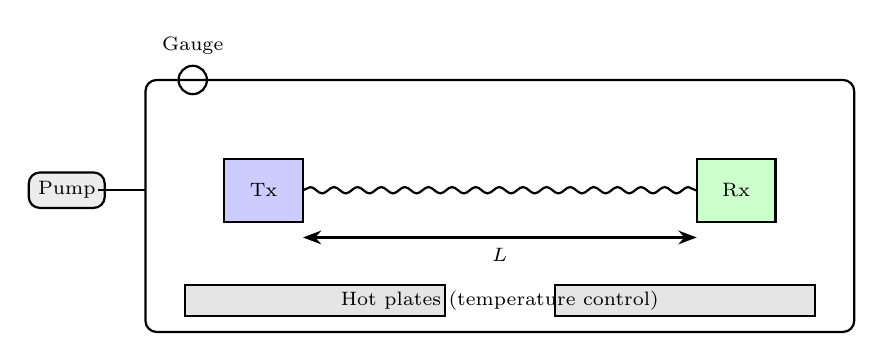
\begin{tikzpicture}[
        every node/.style={font=\scriptsize},
        thick,
        >=Stealth
    ]
    
    % Chamber
    \draw[rounded corners] (0,0) rectangle (9,3.2);
    
    % Hot plates
    \draw[fill=gray!20] (0.5,0.2) rectangle (3.8,0.6);
    \draw[fill=gray!20] (5.2,0.2) rectangle (8.5,0.6);
    \node at (4.5,0.4) {Hot plates (temperature control)};
    
    % Transducers
    \draw[fill=blue!20] (1.0,1.4) rectangle (2.0,2.2);
    \node at (1.5,1.8) {Tx};
    
    \draw[fill=green!20] (7.0,1.4) rectangle (8.0,2.2);
    \node at (7.5,1.8) {Rx};
    
    % Sound wave
    \draw[decorate, decoration={snake, amplitude=0.4mm, segment length=3mm}]
          (2.0,1.8) -- (7.0,1.8);
    
    % Distance L
    \draw[<->] (2.0,1.2) -- (7.0,1.2);
    \node[below] at (4.5,1.2) {$L$};
    
    % Pressure gauge
    \draw (0.6,3.2) circle (0.18);
    \node[above] at (0.6,3.4) {Gauge};
    
    % Vacuum pump
    \node[draw, rounded corners, fill=gray!15] at (-1.0,1.8) {Pump};
    \draw (0,1.8) -- (-0.6,1.8);
    
    \end{tikzpicture}%
    }
    
    \end{frame}

% =========================
% Results: Temperature
% =========================
\begin{frame}{Results: Temperature Dependence}
\begin{columns}
\begin{column}{0.46\textwidth}

\textbf{Observations:}
\begin{itemize}
    \item 30 data points (20--80°C)
    \item Speed increased from \SI{351}{m/s} → \SI{391}{m/s}
    \item Matches $\sqrt{T}$ prediction
\end{itemize}

\vspace{0.2cm}
\textbf{Data Quality:}
\begin{itemize}
    \item Avg. error: \textbf{0.8\%}
    \item Fit quality: $R^2 > 0.999$
\end{itemize}

\end{column}

\begin{column}{0.54\textwidth}
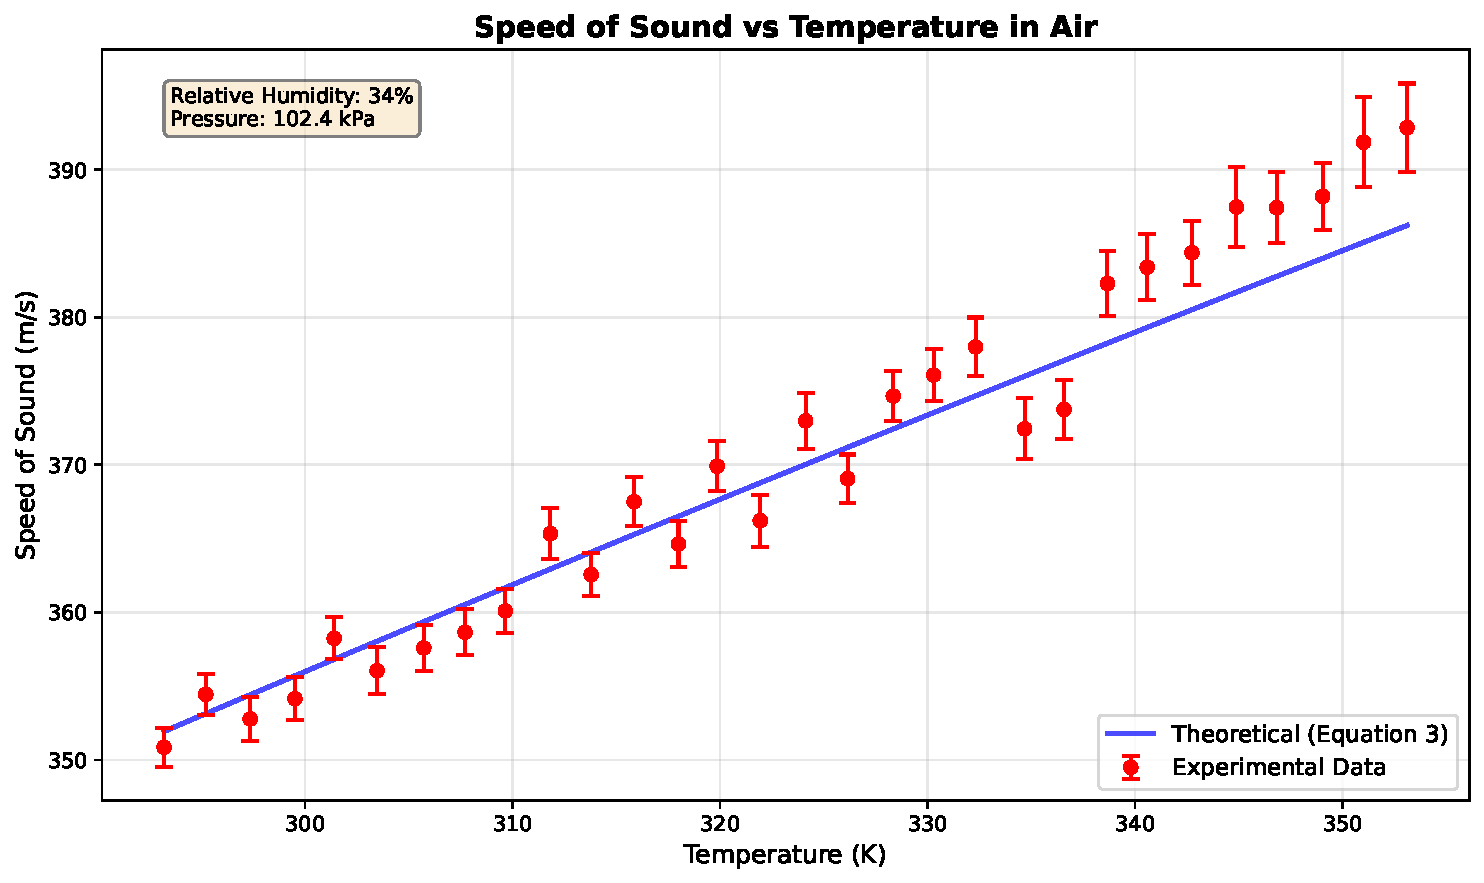
\includegraphics[width=\textwidth]{plots/temperature_dependence.pdf}
\end{column}
\end{columns}
\end{frame}

% =========================
% Results: Pressure
% =========================
\begin{frame}{Results: Pressure Dependence}
\begin{columns}
\begin{column}{0.48\textwidth}

\textbf{Observations:}
\begin{itemize}
    \item 10 measurements (100\%→0.1\% atm)
    \item Temperature fixed at 20°C
    \item Speed remained \textbf{nearly constant}
\end{itemize}

\vspace{0.2cm}
\textbf{Theory:}  
For ideal gas, speed depends only on temperature.

\vspace{0.2cm}
\textbf{Error context:}
\begin{itemize}
    \item Variations $< 2\%$ within uncertainty
    \item Larger fluctuations at $< 1\%$ pressure
\end{itemize}

\end{column}

\begin{column}{0.52\textwidth}
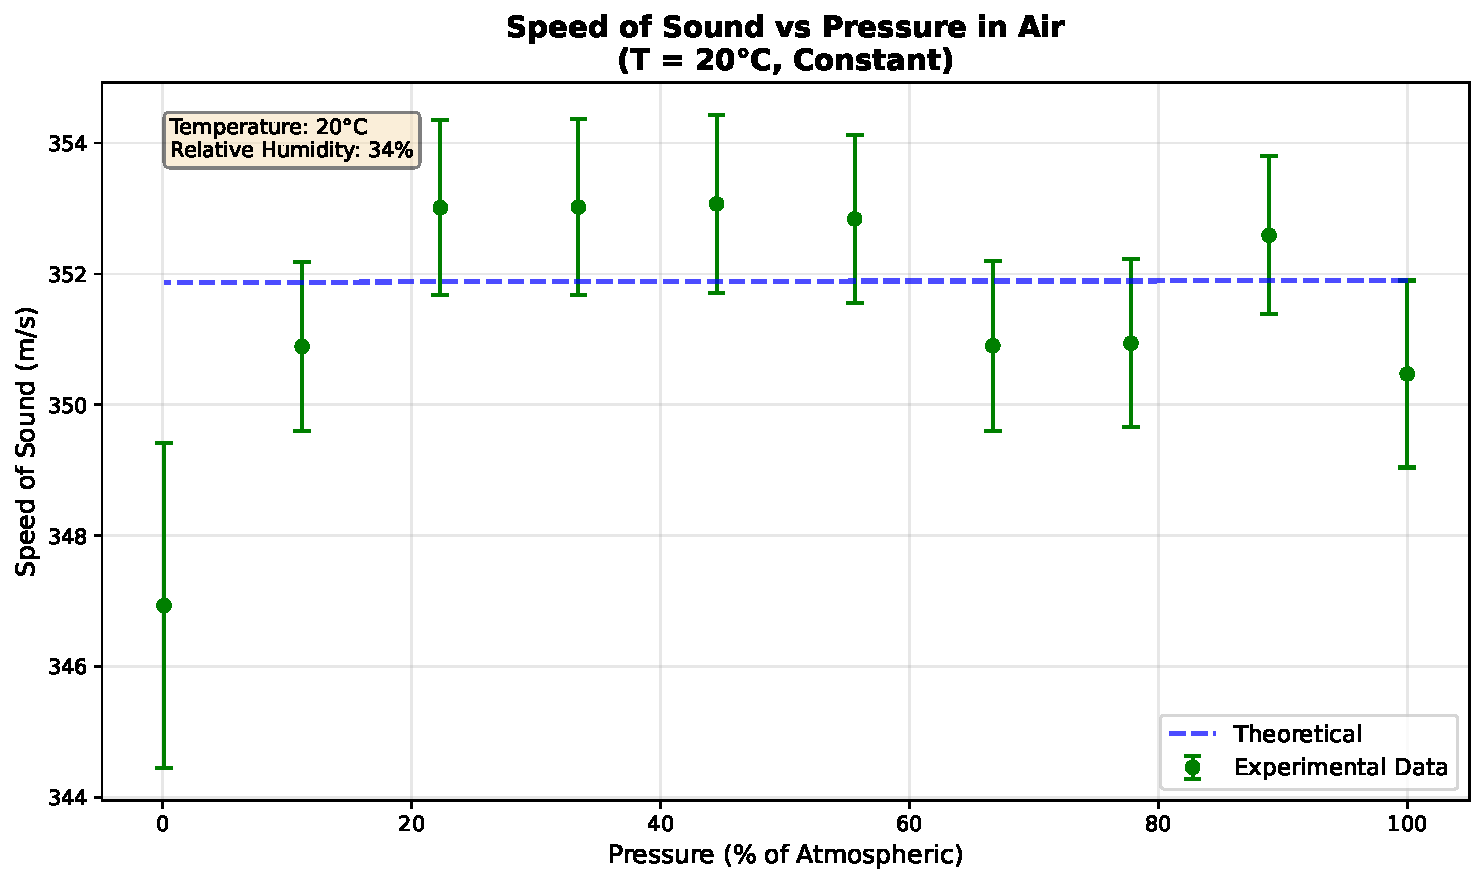
\includegraphics[width=\textwidth]{plots/pressure_dependence.pdf}
\end{column}
\end{columns}
\end{frame}

% =========================
% Error Analysis
% =========================
\begin{frame}{How Good Were Our Results?}
\begin{columns}
\begin{column}{0.5\textwidth}

\textbf{Main error sources:}
\begin{itemize}
    \item \textbf{Measurement:} caliper resolution, frequency accuracy
    \item \textbf{Environment:} temperature drift, pressure instability
    \item \textbf{Detection:} phase difference reading
\end{itemize}

\vspace{0.3cm}
\textbf{Error Trends:}
\begin{itemize}
    \item Low T: 0.4--0.5\%
    \item High T: 1.0--1.5\%
    \item Very low P: $\sim$1.4\%
\end{itemize}

\end{column}

\begin{column}{0.5\textwidth}

\textbf{Experimental Challenges:}
\begin{itemize}
    \item Temperature stability of hot plates
    \item Vacuum chamber limitations at very low pressure
    \item Long thermal equilibration time
\end{itemize}

\vspace{0.4cm}
\textbf{Overall uncertainty:}  
\SI{1.5}{m/s} -- \SI{2.0}{m/s} (0.4--1.5\%)

\end{column}
\end{columns}
\end{frame}

% =========================
% What We Learned
% =========================
\begin{frame}{What We Learned}
\begin{enumerate}
    \item \textbf{Temperature dependence confirmed:} $v \propto \sqrt{T}$
    \item \textbf{Pressure independence verified:} constant within error
    \item \textbf{High precision:} average deviation 0.8\%
    \item \textbf{Physical insight:} sound speed depends on molecular motion
\end{enumerate}

\vspace{0.4cm}
\textbf{Conclusion:}  
Strong alignment between theory and experiment across a wide parameter range.
\end{frame}

% =========================
% Limitations + Future Work
% =========================
\begin{frame}{Limitations \& Future Work}

\textbf{Limitations:}
\begin{itemize}
    \item Equipment-limited temperature range
    \item Difficult to maintain $<1\%$ pressure
    \item Ideal-gas model breaks at high temperatures
\end{itemize}

\vspace{0.4cm}

\textbf{Future Work:}
\begin{itemize}
    \item Explore humidity effects
    \item Test other gases (CO\textsubscript{2}, He)
    \item Improve temperature uniformity
\end{itemize}

\end{frame}

% =========================
% Main Takeaway
% =========================
\begin{frame}{Main Takeaway}
\begin{center}
\Large
\fbox{\parbox{0.83\textwidth}{
\centering
\textbf{\Huge Our Key Finding}\\[0.4cm]
\Large
Sound speed in air \textbf{increases with temperature} ($v \propto \sqrt{T}$)\\[0.2cm]
but is \textbf{independent of pressure} in the ideal gas regime.
}}
\end{center}
\end{frame}

% =========================
% Acknowledgements
% =========================
\begin{frame}{Acknowledgments}

\vspace{0.5cm}
\begin{center}
\Large Thank you!\\[0.3cm]
Questions?
\end{center}

\begin{itemize}
    \tiny
    \item Lab instructors: Kai Wang, Chen Xi
    \item Course instructor: Prof. Changcheng Zheng
    \item Prof. Xiawa Wang's Lab (equipment \& support)
\end{itemize}

\end{frame}

\end{document}